% 20200719
\documentclass[../thesis.tex]{subfiles} %% use packages & commands as this main file
\begin{document}
\section{Result}
Numerical simulation showed stability in biomass densities on destructive harvest systems for both \PoN\ and \PBN\ (Fig.\ref{f:destCarbon}).  After an initial boost of organic carbon accumulation (Fig.\ref{f:destCarbon}A), \phy-only systems had linear accumulation of organic carbon but \pbs\ had its level slightly dropped to a stable level and perpetuated.  The difference in carbon accumulation trend led to non-significant different between \PoN\ systems only after a few days of system establishment (Fig.\ref{f:ydByHarv}A).  We did not observe this pattern in \pbs.

Log distributions for \phy-only systems were stable with much wider yield ranges than \pbs\ regardless of harvest mode (Fig.\ref{f:ydByHarv}B).  On a contrary, most \pbs s yielded 0 \dxdt\ (for both medians and interquartile ranges) with an exception of \PBN\ systems with low harvest interval (median 0.02, IQR [-0.01 - 0.12]\dxdt).  For maximum yield scenarios of each of the four systems, \PoH\ and \PoN\ have similar yield of 345-346\dxdt.  \PBH\ systems had an overall decreased yet fluctuating maximum from 275 ($x$ = 101) to 176 ($x$ = 1001) to 218 ($x$ = 10001) \dxdt.  \PBN\ systems had a decreased and flattened maximum trend from 198 ($x$ = 101) to 66 ($x$ = 1001 and 10001) \dxdt.

Pairwise Wilcox test showed statistical significance for all four systems (\PBH, \PoH, \PBN\ \& \PoN).  Yet in Fig.\ref{f:ydByPara} the pair of \phy-only systems were largely overlapping and the overlap was also observed for the \pbs s.  Hence we concluded that biological significance was only between \phy-only and \pbs s but not across harvest terms within each pair.

Biological parameters for \phy\ (Fig.\ref{f:ydByPara}A-D) had stable influence over \phy-only systems (\PoH\ \& \PoN) in the view of the median.  No parameters had influence on median values for \pbs s (\PBH\ \& \PBN in Fig.\ref{f:ydByPara}A-H).  As for \phy\ biological parameters, only intraspecific interference ($\aP$) had a decreasing effect in a decreasing rate.  Hence density-insensitive \phy\ death rate had much higher productivity than others; maximum yield for all four systems concentrated at the minimal value for this parameter range.  The other three \phy\ parameters (i.e. non-respirable carbon fraction for \phy\ $\ePR$, carbon fraction allocated into biomass for \phy\ $\eP$ and \phy\ growth rate $\gP$) had a stable positive influence on median of \phy-only systems yield fluxes.  Although pairwise Wilcox test showed significance (p $\ll$ 0.01) between \PoH\ and \PoN, the difference may not be biological significant.  The set of four parameters had no observational effect on \pbs s.  The reason was because most of the raw yield from simulations were zeros.  Details were listed later in this section.

Biological parameters for \bac\ (Fig.\ref{f:ydByPara}E-H) had no observable influence over all systems.  Since these four parameters had no mathematical effect on \phy-only systems (equilibrium 3 in Table \ref{t:eqm}), fluctuations from \phy-only systems in Fig.\ref{f:ydByPara}E-H was due to LHS sampling effect.  Yet, it also had no observational effect on \pbs s, probably because of the large number of zero yield scenarios.

The maximum yield scenario for each system were different.  \PoH\ and \PoN\ were very similar and they achieved their own maximum at the same biological parameter combination (Fig.\ref{f:ydByPara}).  \PBH\ had different maximum yield than \PBN\ and their sets of biological parameter combination were different.  Among the LHS samples, \PBH\ achieved its maximum yield (285 \dxdt) when harvest rate was 2101 \dayU.  The set of phytoplankton features was high carbon to biomass conversion efficiency under moderate-high growth rate and minimal population density sensitivity.  Bacterial features were mid-level of carbon to biomass conversion efficiency under moderate-high growth rate and moderate-low death rate.  \PBN\ achieved its maximum yield (198 \dxdt) at a frequent interval (101 \dayU).  Its set of phytoplankton features was similar to that of \PBH\ but different \bac l feature requirement.  A \PBN\ system required high leakage bacteria with very high growth rate and high death rate.  In short, all four systems had similar preferences on phytoplankton.  But if \bac\ was involved, requirement for the best \bac\ was strict and specific based on the designated type of system.

Among the four system sets within the LHS scenarios (1.1 million), feasible (for continuous harvest systems) and favourable (for destructive harvest systems) were counted.  Feasible systems were systems that a biological meaningful carbon density at the stable state of such system were analytically calculated.  For \PoH, 88.3\% (n=971039) were feasible.  On a contrary, only 0.3\% (n=3251) of \PBH\ systems were feasible.  Favourable systems were scenarios that had a net gain of carbon during numerical integration.  99.5\% (n=1094500) \PoN\ systems but 47.0\% (n=517113) \PBN\ systems were favourable.  Compare the number of feasible/favourable systems with the maximum yield (Fig.\ref{f:ydByPara}), it showed \phy-only systems were easy to construct with high yield.  Yet a fit \bac\ candidate could also bring carbon harvest up to high levels.

\begin{figure}[H]
    \centering
    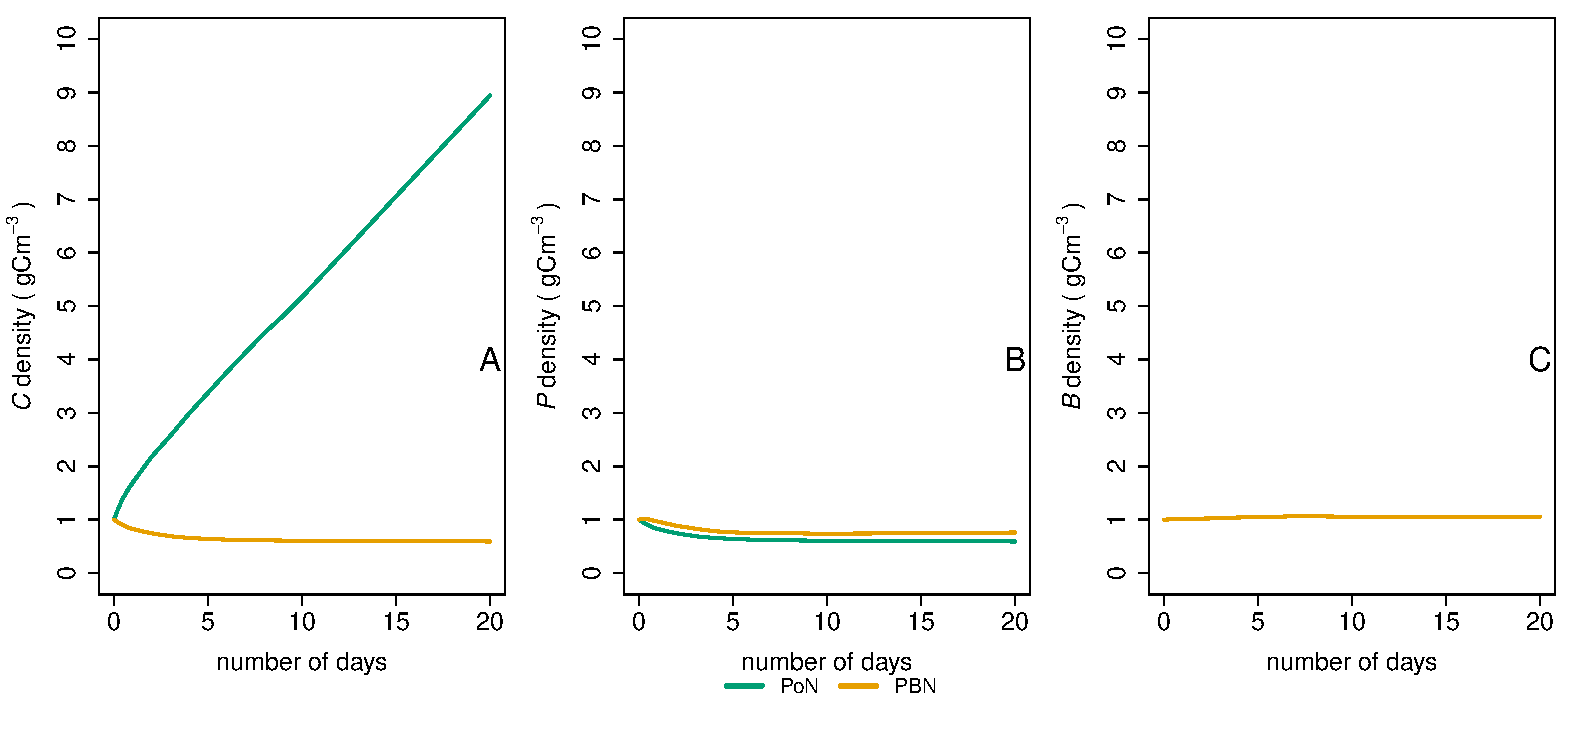
\includegraphics[width=\linewidth]{result/Sample.pdf}
    \caption[Carbon content in a sample destructive system]{Carbon content in a selected destructive system.  $C$, $P$ and $B$ were carbon pools in Fig.\ref{f:model}.  Eq.\ref{eq:PBH} was used with different initial carbon densities to address the \PoN\ and \PBN\ modes.  Biological parameters in this sample system were 0.3158 ($\ePR$), 0.8800 ($\eP$), 1.9152 ($\gP$), 1.5214 ($\eP$), 0.8259 ($\eBR$), 0.6007 ($\eB$), 2.4768 ($\gB$) and 0.4405 ($\mB$).  Initial carbon densities for \PoN\ were [1,1,0]\den\ ($C$, $P$, $B$) and that for \PBN\ were [1,1,1]\den.}
    \label{f:destCarbon}
\end{figure}

\begin{figure}[H]
    \centering
    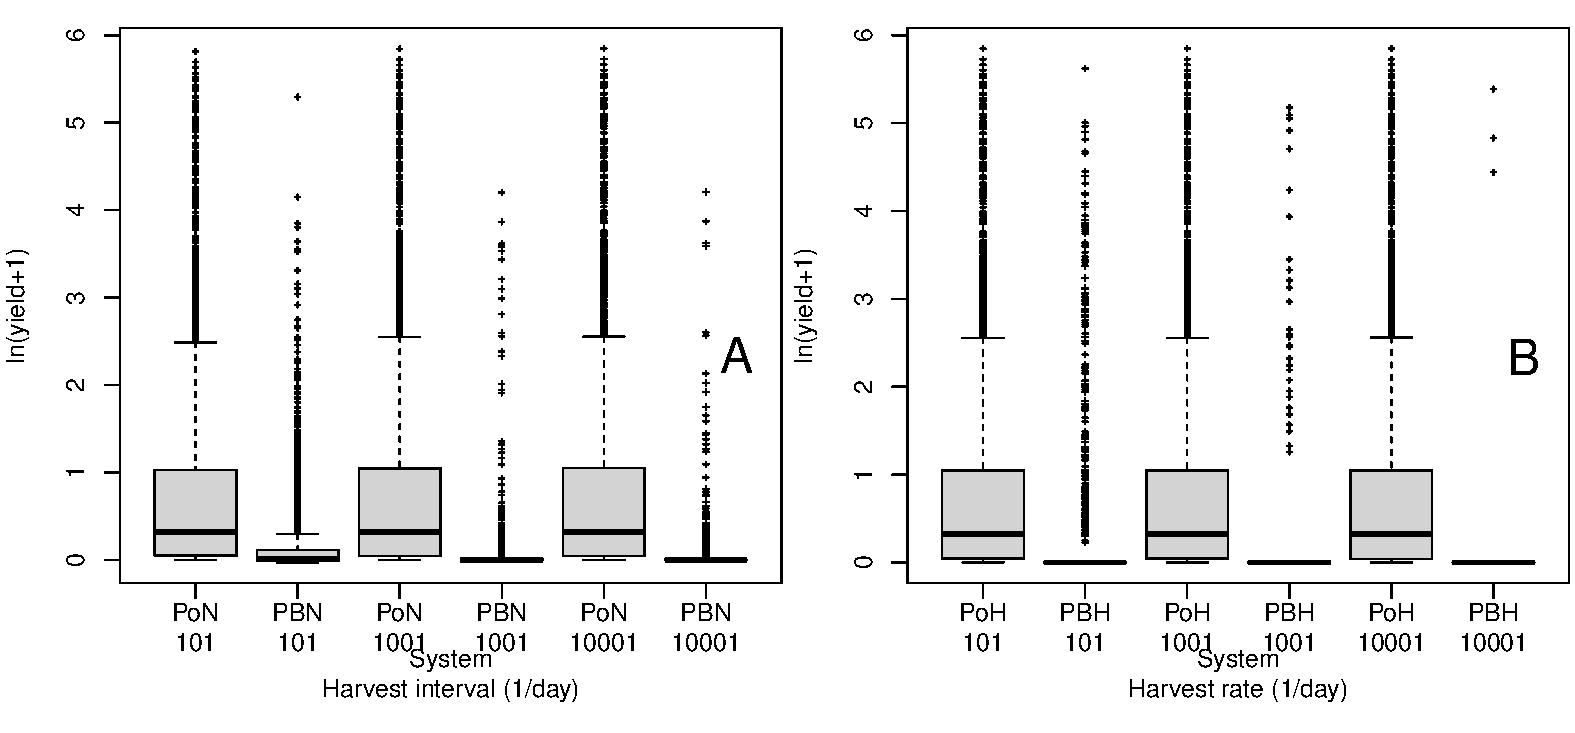
\includegraphics[width=\linewidth]{result/Harvest.pdf}
    \caption[Yield flux distribution by harvest mode]{Log distribution of yield for destructive (subplot A) and continuous (subplot B) harvest modes on selected harvest interval/rates.  (A) Pairwise Wilcox test showed significance (p $\ll$ 0.01) between all except the pair of \PoN\ systems interval 5 and 50 days (p $>$ 0.1).  (B) \Phy-only (\PoH/\PoN) and coexistence (\PBH/\PBN) systems were significantly different (p $\ll$ 0.01).  Significance was also found between \pbs s (p $\ll$ 0.01) but not \phy-only systems (p $>$ 0.1).  Each box represented a sample size of 5500.}
    \label{f:ydByHarv}
\end{figure}

\begin{figure}[H]
    \centering
    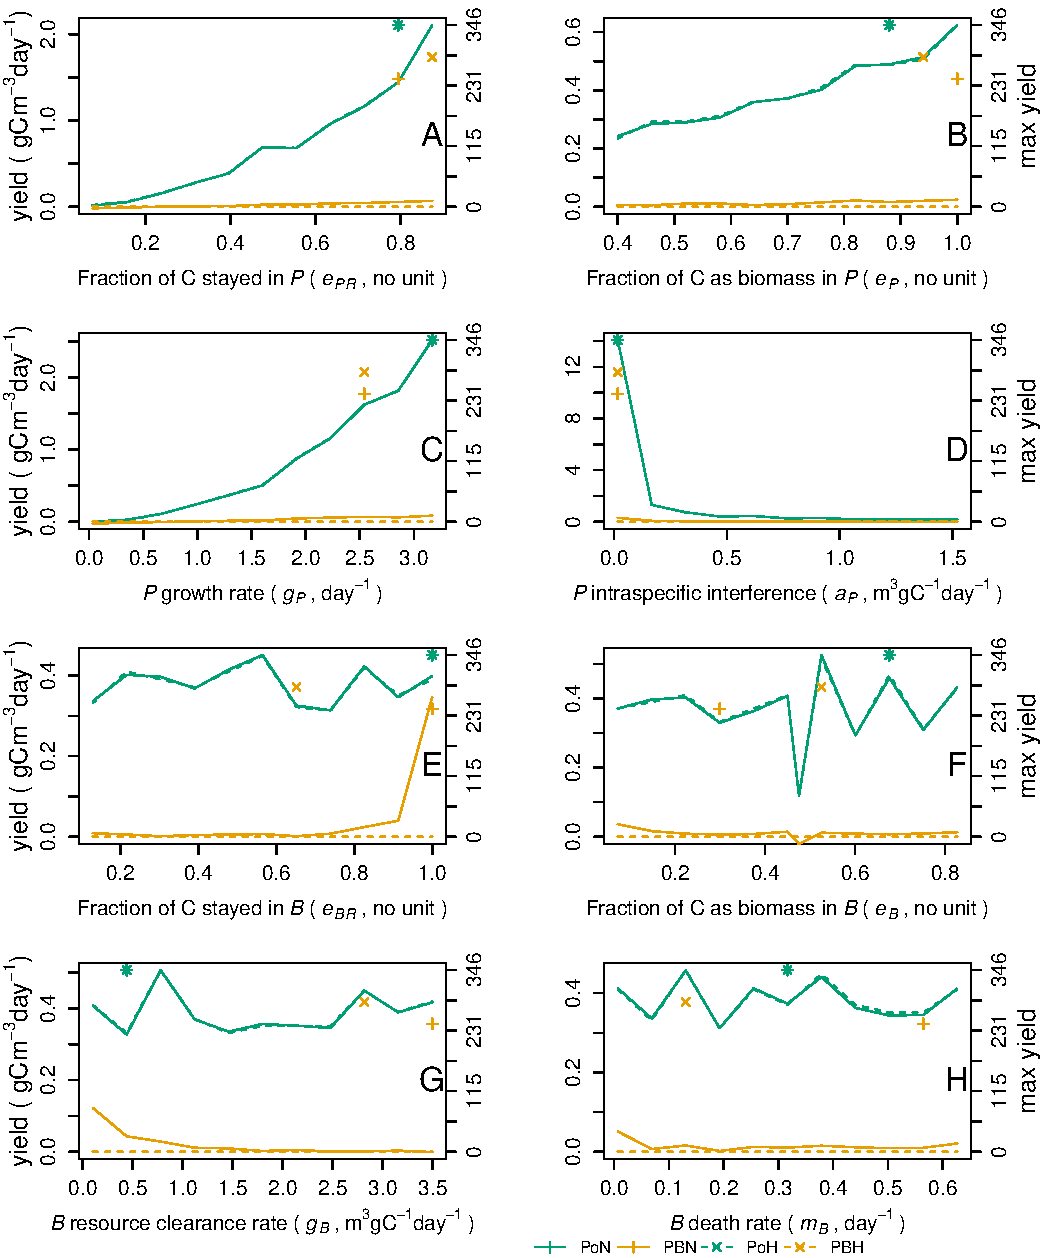
\includegraphics[width=\linewidth]{result/yieldFlux.pdf}
    \caption[Yield flux median in biological parameter space]{Median yield flux (primary axis) and the maximum yield scenario (secondary axis) along respective parameter ranges under a standardised temperature range of \temp.  Each system had an LHS sample size of 1.1 million.  Pairwise Wilcox test showed significance (p $\ll$ 0.01) between all systems.}
    \label{f:ydByPara}
\end{figure}

\end{document}